\subsection{Aufbau}
Zentrales Element des Aufbaus ist ein Helium-Neon Laser der mit einer Wellenlänge von $\lambda = 633\si{\nano \meter}$ auf einen
verschiebbaren Spalt strahlt. Auf Grund der langen Kohärenzlänge von Lasern ist der Abstand zum Spalt ohne Bedeutung.
Das vom Spalt erzeugte Inteferenzmuster wird anschließend auf einen Lichtempfindlichen Detekor projeziert, 
welcher in der Lage ist, durch eine Photoiode, die Intensität mit Hilfe eines Ampermeters auzulesen. Der Abstand zwischen dem Spalt und 
dem Detekor misst $127\si{\cm}$. 
\\
\newline
Die verschieden Spalte werden auf eine Halterung unmittelbar hinter dem Laser angebracht und so ausgerichtet, dass der Lichtstrahl 
genau durch den zum Verusch passenden Spalt läuft. Für den Versuch werden zwei Konfiguartionen der Spalte benutzt. 
Ein einfacher Spalt mit einer Breite von $b_1=?????$ und ein Doppelspalt mit dem Spaltabstand $g=?????$ und der Breite $b_2=????$.
\\ 
\newline
Um die Maxima und Minima des Inteferenzmusters auslesen zu können, ist der Detekor auf eine Schiene montiert. 
Diese Schiene bietet eine Variation von jeweils $25 \si{\mm}$ nach oben und unten und ermöglicht es so die vom Winkel
$\phi$ abhängige Intensität zu messen.
\begin{figure}
    \centering
    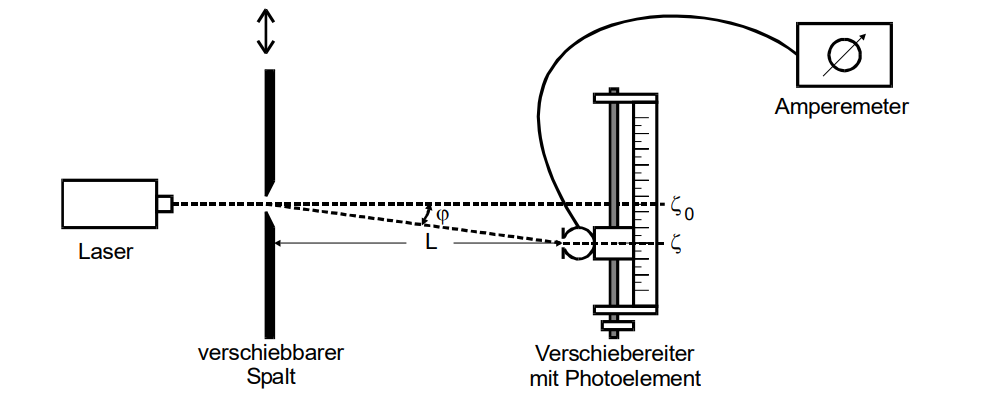
\includegraphics[width=\textwidth]{bilder/aufbau.png}
    \caption{Schematischer Aufabu des Lasers mit verschiebbaren Spalt und Detekor \cite{skript}.} 
    \label{fig:abb1}
\end{figure}
